%%%%%%%%%%%%%%%%%%%%%%%%%%%%%%%%%%%%%%%%%%%%%%%%%%%%%%%%%%%%%%%%%%%%%%%%%%%%%%%
\section{Flujometrías}

De los resultados de la primer otpimización se extrajo una curva de diferencia
de presión vs alzada en diferentes velocidades del motor con el finde de
identificar los puntos de mayor interés para realizar las flujometrías,
tratando de obtener una buena cobertura del rango de funcionamiento de cada
puerto.

% inicialmente se propusieron un total de XXX flujometŕias, sin embargo algunas
% combinaciones de $\l_{v}, \Delta P$ no se pudieron ejecutar hasta la
% convergencia del flujo másico, por lo que se redujo la cantidad de flujometrías
% final a xxx flujometrías, xxx para el puerto de admisión y xxx para el puerto
% de escape, el par  se detalla en la figura XXX y tabla xxx.

Los pares $(\l_{v}, \Delta P)$ se detallan en la figura XXX, en estos puntos se
flujó el puerto para luego se calcular el coeficiente de descarga, obteniendo
la base para generar el mapa de $C_D$ que se utilizará en el próximo paso de
simulación.

Como se mencionó en el apartado~\ref{capitulo:DESARROLLO}, la modificaión
realizada a ICESym para funcionar con un mapa de $C_{D}$ dependiente de dos
variable, requiere que los datos de entrada estén distribuidos en una grilla
rectangular, motivo por el cual a partir de estos valores se utilizó el método
de interpolación por IDW para generar una dicha grilla de $(l_{v}, \Delta P)$
con $C_{D}$ interpolado de los datos conocidos, como se ve en las
figuras~\ref{fig:mapa_cd_admision} y~\ref{fig:mapa_cd_escape}.

\begin{figure}
    \centering
    \begin{subfigure}{0.4\textwidth}
        \centering
        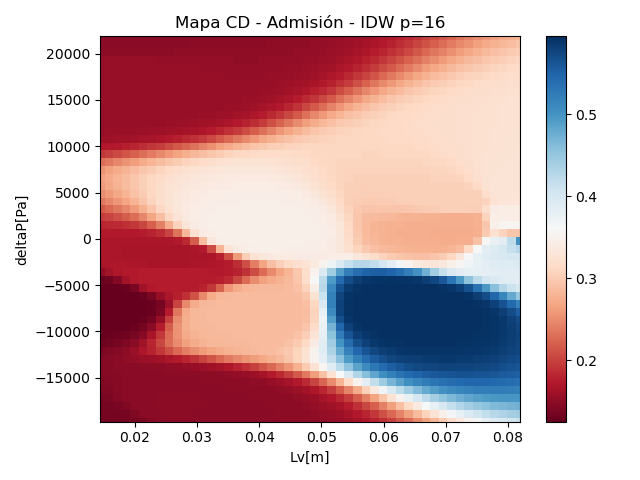
\includegraphics[width=\textwidth]{mapa_cd/idw16_mapa_adm.png}
        \caption{cambiar}
    \end{subfigure}
    \hfill
    \begin{subfigure}{0.4\textwidth}
        \centering
        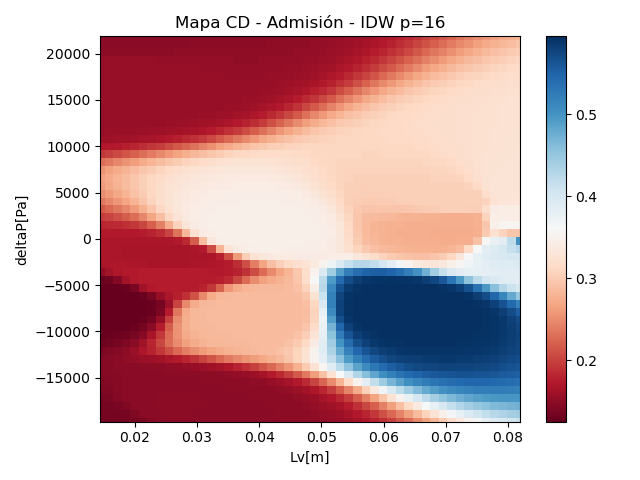
\includegraphics[width=\textwidth]{mapa_cd/idw16_mapa_adm.png}
        \caption{cambiar}
    \end{subfigure}
    \caption{cabmiar}\label{fig:mapa_cd_admision}
\end{figure}

\begin{figure}
    \centering
    \begin{subfigure}{0.4\textwidth}
        \centering
        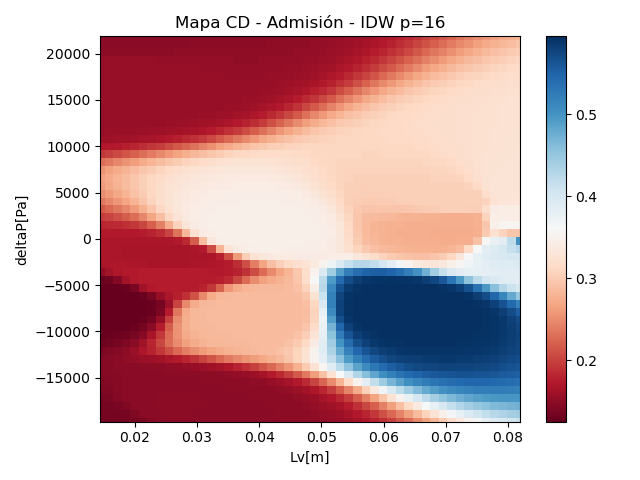
\includegraphics[width=\textwidth]{mapa_cd/idw16_mapa_adm.png}
        \caption{cambiar}
    \end{subfigure}
    \hfill
    \begin{subfigure}{0.4\textwidth}
        \centering
        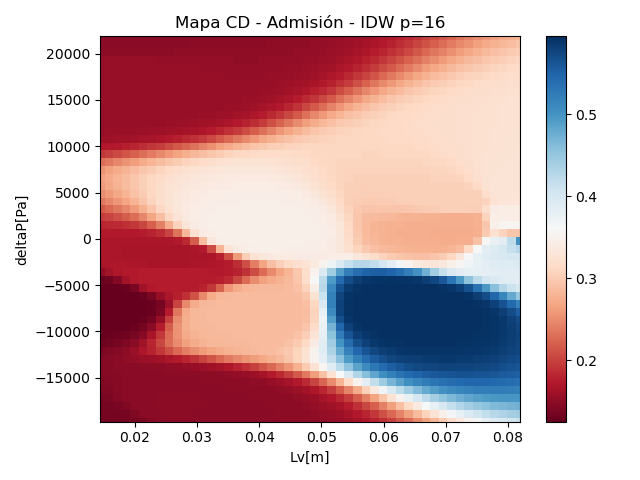
\includegraphics[width=\textwidth]{mapa_cd/idw16_mapa_adm.png}
        \caption{cambiar}
    \end{subfigure}
    \caption{cabmiar}\label{fig:mapa_cd_escape}
\end{figure}

En el mapa del puerto de admisión se observa un máximo para para aperturas del
puerto mayores a 80mm, con $\Delta P$ de entre 1000 Pa a 15000 Pa.
%
El coefiente de descarga máximo es $C_{D}(100mm, 1500Pa) = 0.6$ y corresponde a
la flujometría $N^{\circ} X$, el flujo másico obtenido para este régimen es de
0.02 kg/s, con un a velocidad máxima de xxx m/s en la garganta.
%
El peor valor se es $C_{D}(100mm, 1500Pa) = 0.6$ y corresponde a aperturas
pequeñas del puerto, en la que debido a la reducida sección de pasaje de flujo
se tiene velocidades eleveadas, siendo la máxima de xxx m/s.
%
Para visualizar la diferencia entre uno y otro caso, se representan las líneas
de corriente para ambos casos en la figura
\ref{fig:comparativa_lineas_corriente}.

\begin{figure}
    \centering
    \begin{subfigure}{0.4\textwidth}
        \centering
        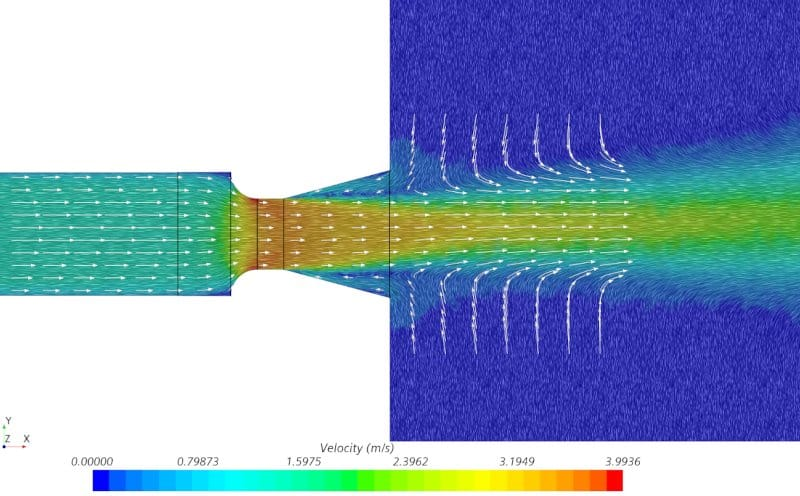
\includegraphics[width=\textwidth]{flujometrias/ejemplo_lineas_corriente.jpg}
        \caption{Valor máximo de $C_{D}$}
    \end{subfigure}
    \hfill
    \begin{subfigure}{0.4\textwidth}
        \centering
        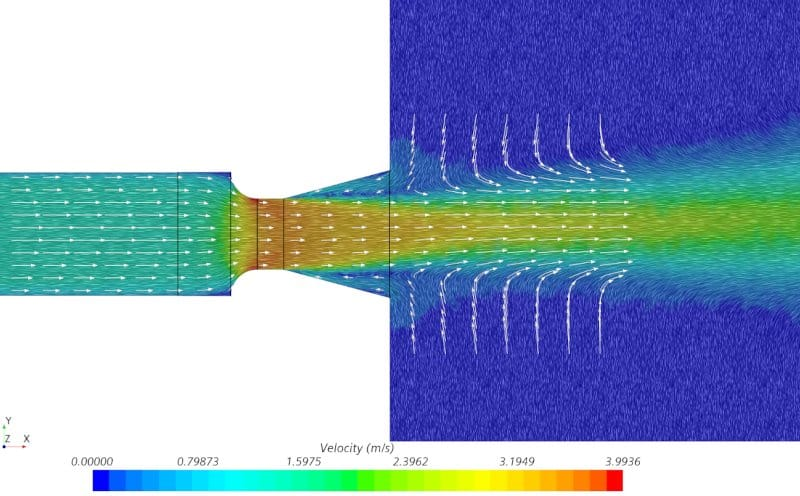
\includegraphics[width=\textwidth]{flujometrias/ejemplo_lineas_corriente.jpg}
        \caption{Valor mínimo de $C_{D}$}
    \end{subfigure}
    \caption{cabmiar}\label{fig:comparativa_lineas_corriente}
\end{figure}

Para el mapa del puerto de escape se observa un máximo para para aperturas del
puerto mayores a 80mm, con $\Delta P$ de entre 1000 Pa a 15000 Pa.
%
El coefiente de descarga máximo es $C_{D}(100mm, 1500Pa) = 0.6$ y corresponde a
la flujometría $N^{\circ} X$, el flujo másico obtenido para este régimen es de
0.02 kg/s, con un a velocidad máxima de 10m/s en la garganta, como se ve en la
figura \ref{fig:admision_10_2000.jpg}.

\begin{figure}
    \centering
    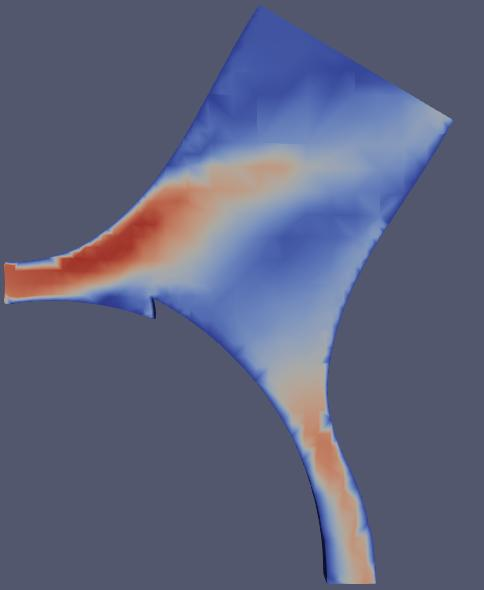
\includegraphics[width=0.7\textwidth]{flujometrias/admision_10_2000.jpg}
    \caption{Puerto de admisión - $10^{\circ}$@2000 RPM}\label{fig:admision_10_2000.jpg}
\end{figure}

El peor valor se es $C_{D}(100mm, 1500Pa) = 0.6$ y corresponde a aperturas
pequeñas del puerto, en la que debido a la reducida sección de pasaje de flujo
se tiene velocidades eleveadas, siendo la máxima de xxx m/s.
%
Para visualizar la diferencia entre uno y otro caso, se representan las líneas
de corriente para ambos casos en la figura \ref{fig:admision_10_2000.jpg}.

\begin{figure}
    \centering
    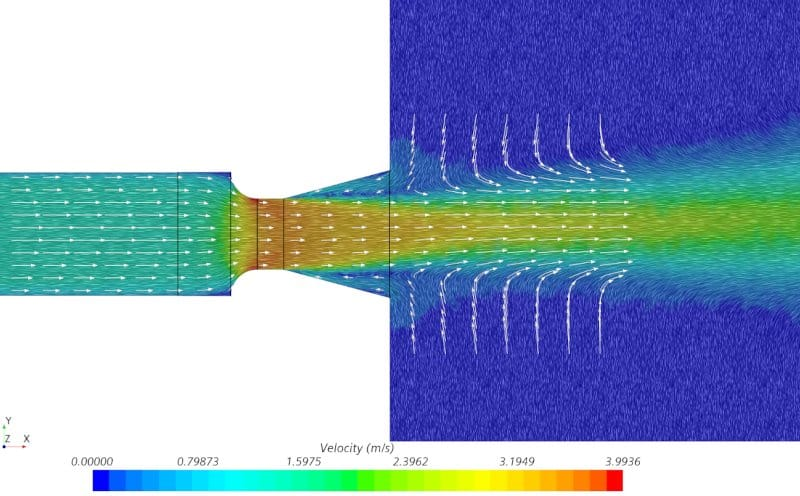
\includegraphics[width=0.7\textwidth]{flujometrias/ejemplo_lineas_corriente.jpg}
    \caption{Puerto de admisión - $10^{\circ}$@2000 RPM}\label{fig:admision_10_2000.jpg}
\end{figure}

En las tablas~\ref{tab:mapa_cd_admision} y~\ref{tab:mapa_cd_escape} se muestran los
resultados de realizar las flujometrías de los puertos de admisión y escape.

\begin{table}
  \centering
    \begin{tabular}{cccc} \toprule
      Caso  & lv        & $\Delta P$    & $C_{D}$   \\ \midrule
      0     & 0.016826  & -100331.39    &  0.213882 \\
      0     & 0.106775  & 5723.72       &  0.489375 \\
      0     & 0.016826  & -263797.72    &  0.011021 \\
      0     & 0.106775  & -3296.18      &  0.803197 \\
      0     & 0.016826  & -652902.78    &  0.011106 \\
      0     & 0.106775  & -9613.29      &  0.815804 \\
      0     & 0.016826  & -513568.73    &  0.011280 \\
      0     & 0.106775  & -3232.97      &  0.813186 \\
      1     & 0.026960  & -116996.12    &  0.375219 \\
      1     & 0.096641  & -3643.9       &  0.878414 \\
      1     & 0.026960  & -237724.11    &  0.018632 \\
      1     & 0.096641  & -6684.11      &  0.867774 \\
      1     &  0.02696  & -496509.46    &  0.111212 \\
      1     &  0.09664  & -18256.20     &  0.805830 \\
      1     & 0.026960  & -237724.11    &  0.022716 \\
      1     & 0.096641  & -6684.11      &  0.862647 \\
      2     & 0.047228  & -49343.47     &  0.541857 \\
      2     & 0.076373  & -5712.86      &  0.918061 \\
      2     & 0.047228  & -109348.67    &  0.487137 \\
      2     & 0.076373  & -17090.38     &  0.914182 \\
      3     & 0.067496  & 13.83         &  0.696967 \\
      3     & 0.071759  & -134.24       &  0.707263 \\
      3     & 0.067496  & -100073.52    &  0.731100 \\
      3     & 0.071759  & -24077.34     &  0.723965 \\
      4     & 0.075750  & -11793.31     &  0.946392 \\
      4     & 0.087764  & -33418.12     &  0.235717 \\
      4     & 0.087764  & -10715.70     &  0.221632 \\
      4     & 0.075750  & -5167.81      &  0.897169 \\
      6     & 0.123601  & -73.94        &  0.878522 \\ \bottomrule
    \end{tabular}
  \caption{Mapa de $C_D$ del puerto de escape} \label{tab:mapa_cd_escape}
\end{table}

\begin{table}
  \centering
  \begin{tabular}{cccc} \toprule
      Caso  & lv        & $\Delta P$    & $C_{D}$   \\ \midrule
      0     & 0.014432  & -6574.97      &  0.206543 \\
      0     & 0.081937  & -87.24        &  0.828822 \\
      0     & 0.014432  & 21856.29      &  0.243975 \\
      0     & 0.081937  & -573.65       &  0.738459 \\
      0     & 0.014432  & -19738.67     &  0.222406 \\
      0     & 0.081937  & 519.60        &  0.487115 \\
      0     & 0.081937  & 1571.95       &  0.587277 \\
      0     & 0.014432  & 18077.97      &  0.256415 \\
      0     & 0.014432  & 2668.61       &  0.247292 \\
      0     & 0.081937  & 0.98          &  0.025970 \\
      2     & 0.062951  & -297.79       &  0.816487 \\
      2     & 0.081937  & 292.92        &  0.466147 \\
      2     & 0.062951  & -7374.88      &  0.980617 \\
      2     & 0.081937  & 4953.85       &  0.541619 \\
      3     & 0.071763  & 4092.13       &  0.501641 \\
      3     & 0.025832  & -3689.81      &  0.289852 \\
      4     & 0.069767  & -789.00       &  0.615690 \\
      4     & 0.069767  & 7869.92       &  0.599348 \\
      4     & 0.005564  & -12539.15     &  0.534555 \\
      4     & 0.005564  & -10091.84     &  0.583979 \\ \bottomrule
    \end{tabular}
  \caption{Mapa de $C_d$ del puerto de Admisión} \label{tab:mapa_cd_admision}
\end{table}


La geometría obtenida luego de realizar la optimización con los mapas de $C_D$
incorporados a la simulación de ICESym se muestra en la figura \ref{fig:geom_nueva}.
%
Se puede ver que la geometría es similar a la inicial, siendo el puerto de
admisión algo menor en cuanto a diámetro que en el caso inicial.

Como es de esperarse, incorporar estos mapa al modelo del motor tiene un efecto
en el comportamiento del mismo, esto se puede observar principalmente en las
curvas de presión del motor.

\subsection{Mapa de $C_D$}
%
Para obtener el mapa se tomaran valores de flujo másico en las combinaciones de
$(\Delta P, l_v)$ que están indicadas en la tabla~\ref{tab:casos}.
%
% En la figura \ref{fig:flujometrias} se ve que se eligieron más cantidad de
% muestreos en las zonas donde hay mayores cambios de presión.
%
% La figura \ref{fig:flujometrias} fué obtenida a partir de los resultados del
% simulador ICESym, restando para las velocidades seleccionadas la presión de la
% cámara a la presión en la boca del puerto.

\begin{figure}
    \centering
    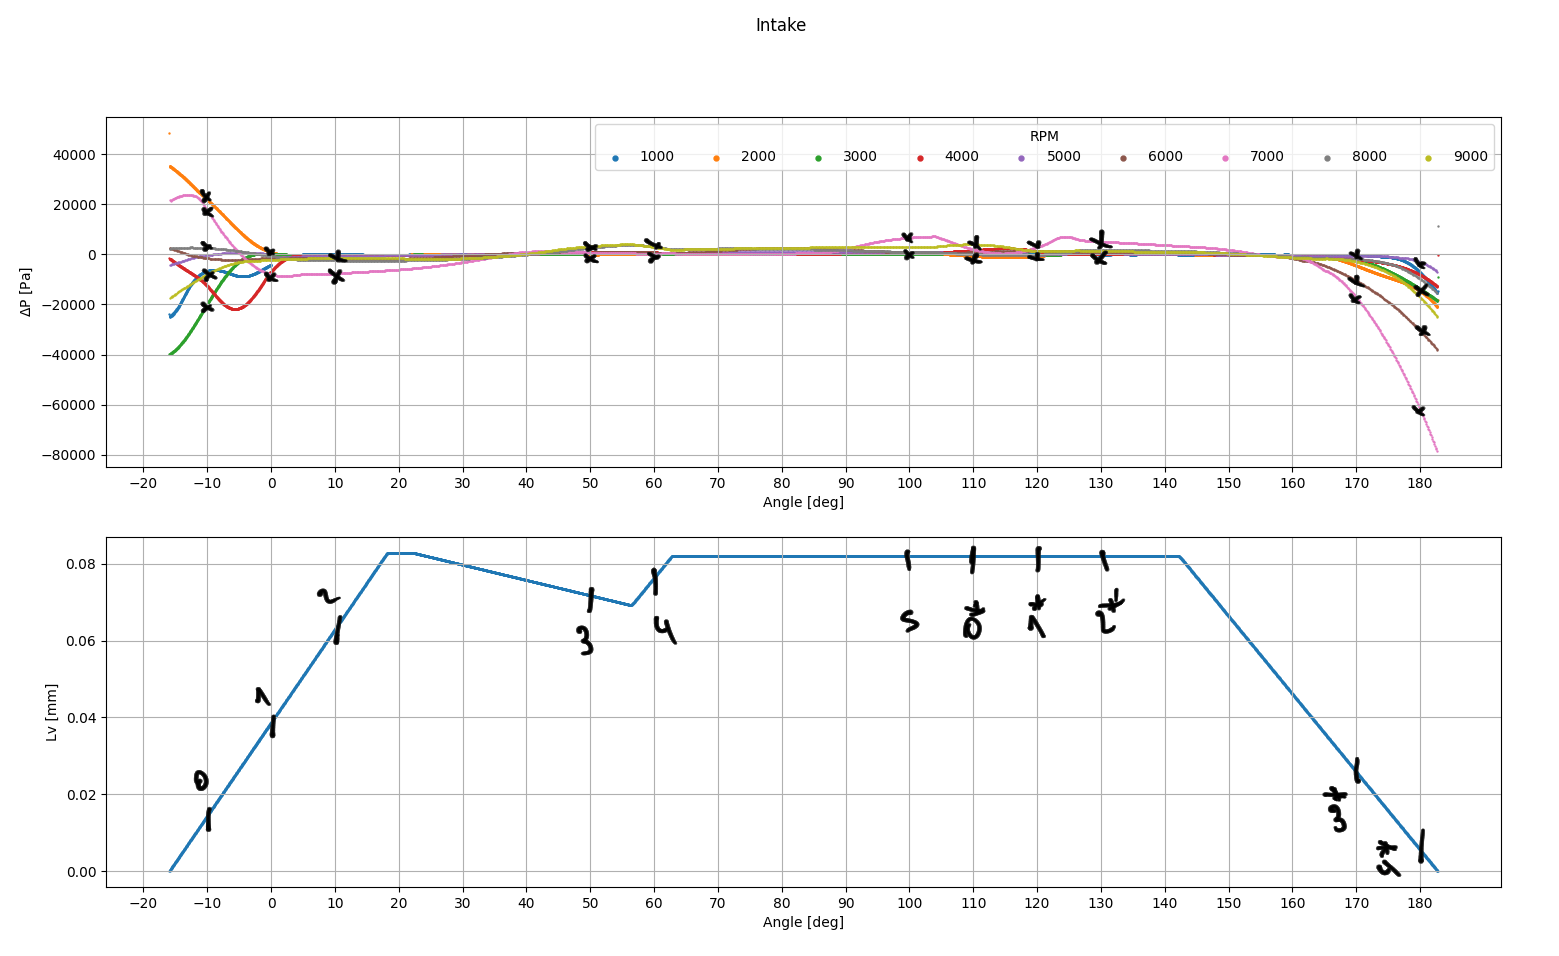
\includegraphics[width=1\textwidth]{flujometrias_admision.png}
    \caption{Flujometrías para el puerto de Admisión}\label{fig:flujometrias}
\end{figure}

\begin{table}
    \centering
    \begin{tabular}{rll} \toprule
        Caso & Ángulos  & Velocidades (rpm) \\ \midrule
        0    & -10, 110 & 1000, 2000, 3000, 7000, 8000 \\
        1    & 0, 120   & 2000, 7000 \\
        2    & 10, 130  & 2000, 7000 \\
        3    & 50, 170  & 3000, 7000, 9000 \\
        4    & 60, 180  & 3000, 5000, 6000, 7000 \\
        5    & 95       & 1000, 7000\\ \bottomrule
    \end{tabular}
    \caption{Flujometrías a realizar}\label{tab:casos}
\end{table}

Como se ve en la Figura~\ref{fig:flujometrias}, los puntos a evaluar son los
listados en la Tabla~\ref{tab:casos}.



\begin{figure}[h]
    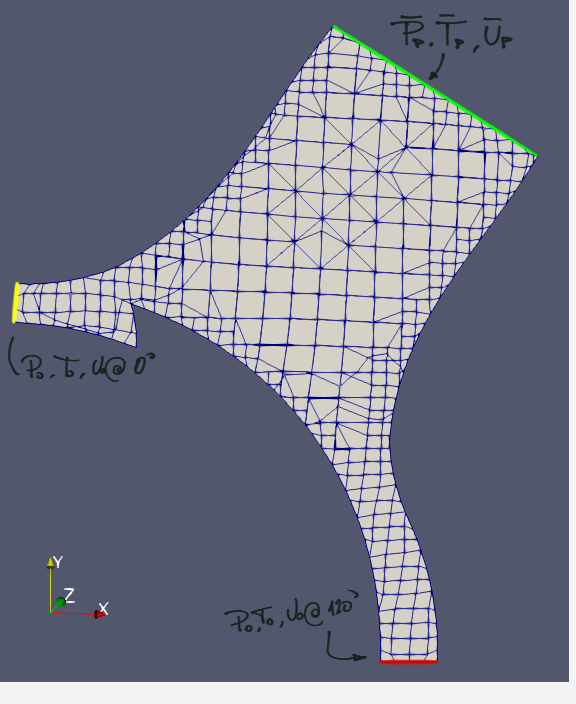
\includegraphics[width=0.8\textwidth]{caso_1-cc.png}
    \caption{Condiciones de borde}\label{fig:geom}
\end{figure}

Dentro del volumen de control, el campo de presiones se inicializa con el valor
medio de presiones de las cámaras y el campo de velocidades se hace
inicialmente (0,0,0).
%
El mapa de $C_D$ obetnido a partir de las flujoemtrías se lista en la
tabla~\ref{tab:mapaAdm} y~\ref{tab:mapaEsc} para los mapas de admisión y escape
respectivamente.


\begin{table}
  \parbox{.45\linewidth}{
  \centering
  \begin{tabular}{rccc}\toprule
    Item & $L_v[m]$ & $\Delta P[Pa]$ & $C_D$ \\ \midrule
    \lua{tex.print(mapaCd(myData.admision))}
    \bottomrule
    \end{tabular}
  \caption{Mapa $C_D$ del puerto de Admisión}\label{tab:mapaAdm}
  }
\hfill
\parbox{.45\linewidth}{
  \centering
  \begin{tabular}{rccc}\toprule
    Item & $L_v[m]$ & $\Delta P[Pa]$ & $C_D$ \\ \midrule
    \lua{tex.print(mapaCd(myData.escape))}
    \bottomrule
    \end{tabular}
  \caption{Mapa $C_D$ del puerto de Escape}\label{tab:mapaEsc}
}
\end{table}
